% pdflatex paper.tex
% bibtex paper

\documentclass[12pt]{article}

\usepackage{scicite}
\usepackage{times}
\usepackage{xcolor}
\usepackage{graphicx}
\usepackage{subcaption}
\usepackage{booktabs}
\usepackage{hyperref}

\topmargin 0.0cm
\oddsidemargin 0.2cm
\textwidth 16cm 
\textheight 21cm
\footskip 1.0cm

\newcommand{\note}[1]{{\color{red} [\bf{#1}]}}
\def\v#1{\bm{#1}}

\newenvironment{sciabstract}{%
\begin{quote} \bf}
{\end{quote}}

\title{The Gold Standard and its Discontents: Simulation Suggests that
  Current Clinical Trial Methods are Very Inefficient}

\author
{Jeff Shrager,$^{1,2\ast}$, Asher Wasserman,$^{1}$
\\
\normalsize{$^{1}$xCures, Inc.}\\
\normalsize{$^{2}$Stanford University, Symbolic Systems Program (adjunct)}\\
\\
\normalsize{$^\ast$Address correspondence to: jshrager@stanford.edu}
}

\date{}

\begin{document} 

\baselineskip24pt 
\maketitle 

\begin{sciabstract}

Adaptive trials are now mainstream science. Recently, researchers have
taken the adaptive trial concept to its natural conclusion, proposing
what we call "Global Cumulative Treatment
Analysis"\cite{shrager_theoretical_2013, shrager_rapid_2014}. Similar
to the adaptive trial, decision making and data collection and
analysis in the GCTA are continuous and integrated, and treatments are
ranked in accord with the statistics of this information, combined
with what offers the most information gain. Where GCTA differs from an
adaptive trial, or, for that matter, from any trial design, is that
all patients are implicitly participants in the GCTA process,
regardless of whether they are formally enrolled in a trial. This
paper reports simulation results that suggest that GCTA-like treatment
validation can be much more efficient than current clinical trial
practice.

\end{sciabstract}

\clearpage

\begin{quote}
 “Every practicing physician conducts clinical trials daily as he is seeing patients.”
 -- T.C. Chalmers, 1981
\end{quote}

\section*{Introduction}

Adaptive trials are now mainstream science \cite{Galloetal2006,
  Fioreetal2011, Kimetal2011; Berry, 2012; DAvolioetal2012}, and more
complex adaptive designs are being analyzed (e.g., Cai,etal2013),
including ones that blur the distinction between classical phases
(e.g., Berry, 2012). Although adaptive designs vary widely, their
defining feature is that the particular treatment regimen that a
patient is assigned to will vary depending upon the specific
characteristics that describe that patient, combined with the running
data regarding the performance of all arms. Just as in a classical
randomized controlled trial (RCT) it is only statistically the case
that a given patient will be placed into the treatment regimen that is
most appropriate for them. However, in the adaptive case, this
probability is updated continuously as data come in from all patients
in every arm.

Recently, researchers have taken the adaptive trial concept to its
natural conclusion, proposing what we will call “Global Cumulative
Treatment Analysis” (GCTA) \cite{VickersandScardino2009, Huber2013,
  ShragerandTenenbaum2011, TenenbaumandShrager2011}. In GCTA, just as
in an adaptive trial, decision making and data collection and analysis
are continuous and integrated; all available performance data for
every possible treatment regimen is taken into account at every
decision point for every patient. Similarly, like an adaptive trial,
treatment regimens are ranked in accord with the statistics of all
this information, combined with what offers the most information gain,
both for the patient at hand, and for every similar patient. Where
GCTA differs from an adaptive trial, or, for that matter, from any
trial design, is that all patients are implicitly participants in the
GCTA process, regardless of whether they are formally enrolled in a
trial.

Adaptive trials utilize a different method for computing choices than
an RCT, specifically, in accord with the statistics of the ongoing
trial. But otherwise, just as in an RCT, there is a clear distinction
made between being in a trial or not (i.e., this is still within the
“normal treatment”, model), and once in the trial, one is assigned to
a particular treatment regimen and remains with that treatment
regimen. This is, in fact, a stricter restriction that results from
being enrolled in a trial than not being enrolled in one: Trials, even
adaptive ones, require that patients either remain on the assigned
treatment regimen, or drop out of the trial. As we shall see, this is
a very significant difference between trials of any sort, and the GCTA
process.

Where the GCTA process differs from all the foregoing is, first, all
treatment regimens are available to all patients at all times;
although most of the time the statistics of experimental treatments
for typical patients will be ranked very low. Secondly, unlike either
an RCT or adaptive trial, but more like off-trial treatment, decision
making for each patient goes on continuously.  However, unlike
off-trial treatment, this decision making takes into account all the
available performance data over all treatment regimens and all
patients, including current ones. The other thing that makes the GCTA
process unique is that, again, more like off-trial treatment than like
a trial, when there are no acceptable choices at all (circle “C”), one
is free, indeed, encouraged, to undertake whatever analytical and
treatment measures one can afford, and that data as well is fed back
into the process. We represent this option (“C”) by a circle with
arrows to emphasize that what goes on here can be quite detailed
dissection of the disease process (e.g., Blau and Liakopoulou, 2013),
which can, within this cycle, involve complex omics, analysis, tumor
boards, and so on. The issue from the present standpoint is not what
specifically happens here, but that it is important that the data,
what is decided, and why, are returned to the data stream so that
near-future patients with similar characteristics can benefit from the
findings and decision making inside this subanalytical process.

GCTA process relies upon a very carefully worked out choice ranking
algorithm (box “A”), which we call the Adaptive Decision
Algorithm. Below we analyze several critical issues surrounding this
algorithm.

It is important to highlight the difference between the GCTA approach
and a “big data/data mining” approach to treatment discovery
and validation. In the GCTA approach, patients’ choices are ranked at
the point of care by a combination of the available information,
combined with an estimate of the amount of information that can be
obtained by ranking some choices over others, in careful accord with
the available evidence. Consider, for example, the equipoise case
where there is no information at all to distinguish between two treatment regimens,
that is, they are at 50/50 (or 1:1) with one another. In this case the
Big Data/Data Mining approach expects there to be a random assortment of applications,
and expects to be able to take advantage of the resulting data to
demonstrate which treatment regimen performs better. In a perfectly efficient and
transparent information economy, this might be the case, but we do not
live in that world. The GCTA approach explicitly biases the treatment regimen
rankings offered to a given patient to ensure that the appropriate
level of experimental variability is injected into the distribution of
patients with given characteristics. The GCTA approach expects that
there will be surprises, but when such surprises happen – when a
patient does not respond as expected (in either direction) – we can
utilize the methods of precision medicine (or, more generally, just
detailed analysis by whatever means) to dissect these cases in more
detail. The Big Data/Data Mining approach has no expectations, and so there is no such
thing as a surprise to it, except post hoc when it may be too late to
go back and dissect the surprise, or, more importantly, change the
course of treatment for that patient, if desired.

Numerous theoretical (i.e., statistical) issues arise in the design of
a GCTA and the details of the adaptive decision algorithm. There are,
of course, numerous practical and ethical issues as well, but we focus
here primarily on the theoretical issues. Whereas we know that these
algorithms will be based upon Bayesian statistics, there remain
numerous open questions as to the details of what should happen in
certain common situations. We enumerate a number of such situations
below, along with some preliminary thoughts on how they might be
approached. Although we have tried to deal with these issues somewhat
separately, they obviously interact with one another. In some cases I
have pointed out this interaction and some of the implications, but in
no case have we tried to describe the whole multi-dimensional problem,
nor provide a covering solution. My goal here is to open this
conversation, not to offer final solutions.

\section*{Theoretical Issues in Global Cummulative Treatment Analysis}

Shrager \cite{shrager_theoretical_2013} identified a number of issues
that need to be decided, or at least considered in the design of a
full GCTA. 

\paragraph*{Changing Treatments Midcourse:}

What is the right thing to recommend to patients who are in the middle
of a complex treatment regimen (treatment regimen) when their
treatment regimen is determined to be futile, or a different one is
deemed superior? Similarly, when a new treatment regimen is admitted
whose priors suggest that it might be superior to some of those
already under analysis, under what circumstances should any patients
be transitioned to this new treatment? What can we learn from what
patients do in this case?  (We assume, without repeating the
phrase, that: "What can we learn from what patients do in this case?"
is implicit in each of the following points.)

In the GCTA process patients (with advice from physicians) are making
decisions about their treatment regimen on a continuous
basis. Physicians, in turn are guided by the adaptive decision
algorithm (adaptive decision algorithm).  When the adaptive decision
algorithm determines that a particular treatment regimen is futile, it
is probably in the patients' best interest to transition them to a
new, presumably superior treatment regimen. Once the possibility of
treatment transition is accepted, there are numerous interesting
implications for decision making and analysis. The treatment regimen
to which they should move ought most likely be controlled by the same
adaptive randomization algorithm used in preliminary intake, but, of
course, informed by the new background that this patient has
previously been under another treatment regimen; that is, the simplest
thing to do is to treat this patient as through they are presenting
for the fist time, although with newly expanded historical
information. One theoretical question is: Should an adjustment be made
to the forward-going statistical information generated by this patient
to account for biases introduced by the patient having been already
guided by the adaptive decision algorithm previously? This interacts
with the problem of complex treatment dynamics, esp. regarding
sequential treatments, discussed in more detail below. In computing
the transition choices for this patient, there may be evidence
regarding specific changes in regimen, for example because a patient
was not able to handle a particular treatment, and so there may be
some evidence already regarding this specific transition. Regardless,
such transitions offer us both additional data for the new treatment
regimen to which they transition, as well as additional data regarding
patients having been transitioned from the futile treatment regimen to
new ones. It may be advisable to make such transitions in an
incremental manner, for example, transitioning a handful of patients
to a number of alternative treatment regimens and observing their
performance, and then resorting them as evidence accrues regarding
these transitions.

\paragraph*{On the Priors for New Treatments}

What are the appropriate priors for new treatment regimens or
biomarker configurations that come online?  Priors are, as usual, a
central point of contention in Bayesian methods. There are several
obvious simple ways to determine priors for new treatment regimens (or
biomarker configurations); for example, Spieghalter, et al.  devote 40
page on the topic, and propose methods ranging from non-informative to
expertelicitation. The easy non-informative default is somewhat
problematic because such priors are defined as non-informative with
respect to some specific universe of information. For example, once
there is some information regarding treatment regimens that have been
under analysis for some time, it is likely that the only reason that
one would put forward the new treatment regimen is that the proponents
have some prior reason to believe that it may be superior, or at least
as good as, the current best contending treatment regimen. It might
make sense, therefore, that the priors for the new treatment regimen
be set to match the distribution of the current best contender, at
least. This suggests that expert elicitation is possibly a better
method than non-informative prior setting, although it, of course, has
many issues of its own regarding expert bias. Certainly, as well, one
would wish to utilize any available information from prior clinical
experience with this treatment regimen, such as that available from
toxicological, animal, or human dosing studies.

\paragraph*{What to Recommend for Partial Targets}

When a new biomarker configuration is admitted, or an old one
rejected, or a new marker deemed evidently related (or unrelated) to a
specific treatment regimen, what do we recommend that patients with
and without that biomarker configuration, and in or out of the related
treatment regimens, do? What about patients whose biomarker
configuration overlaps, but is not exactly the same as a new or
retired biomarker configuration?

The introduction of a new biomarker, or, more generally, the discovery
of a new relationship between a biomarker configuration (biomarker
configuration) and a treatment (hereafter called a biomarker
configuration treatment regimen: Biomarker Configuration Treatment
Relationship), is a more complex case than the change in the state of
belief of the efficacy of a treatment regimen. A given patient may
fall under a specific biomarker configuration treatment regimen or
not, or a combination of biomarker configuration treatment regimens,
or may have a biomarker configuration that is similar to some degree
(i.e., in some metric space) to the biomarker configuration in a
particular biomarker configuration treatment regimen. Moreover, as a
result of changes in the belief state with regard to various biomarker
configuration treatment regimens, a particular patient may find him or
herself (somewhat suddenly) undertaking the wrong treatment regimen,
similar to the situation in question 1, above, but in the very much
higher dimensional, and likely quite sparse and lumpy, space of
molecular measures (more generally, patient characteristic vectors;
PCVs). The simplest approach is, of course, an algorithm akin to
nearest neighbor selection, but there are many other options (and
parameters to set within each). Which is best for the expected
distribution of PCVs will almost certainly require modeling to answer.

\paragraph*{Dealing with Complex Mutational Dynamics}

How should we deal with complex disease dynamics such as mutational
escape recurrence in cancer? For example, a treatment that performs
poorly in the short term might be better in the long run because it
leads to less mutational escape and/or resistance to repeated or other
treatments.

The successful operation of adaptive trials depends upon obtaining
high quality outcomes (or proxy biomarkers for outcomes) as rapidly as
possible. In a relatively slow disease, like most cancers, therefore,
instead of waiting for “final” outcomes (usually something like 5
years disease free), proxy (or surrogate1 ) measures are almost always
used, for example, tumor load or PSA status, which can be assessed
right away through direct measurement, and moreover, tracked. However,
unless the measure being used is a validated proxy – that is,
something that has been shown to be highly correlated with the desired
outcome – there is always the possibility of playing an early false
positive. Moreover, because the adaptive decision algorithm will tend
to remove patients from near term underperforming treatment regimens
to near term better performing ones, at least according to the
surrogate measures, the data that would offer the opportunity to
discover a “late winner” is slowly (or sometimes rapidly!)
depleted. We know that this could be a problem for some cancers (and
possibly other disease), where recurrence has been observed to be more
aggressive when the tumor is aggressively treated early on with only
partly effective drugs (e.g., Nahtaetal2006).

How do we cope with the complexities and time dynamics of complex
treatments that take place over months or years?  Treatment regimens
(treatment regimens) in most diseases, and especially in diseases such as cancer,
often extend over weeks or months, and comprise multiple cycles of
treatments of various sorts.  Aside from there being innumerable
parameters involved in such a treatment, most of which we hope are not
very sensitively correlated with outcomes, the duration of such
treatments complicates the data collection of proxy/surrogate
measures, as well as the concept of decision point. On the one hand we
might say that as much data should be captured as soon as possible,
and every moment is a potential decision point, but there is certain
to be variability, and most treatments have high short term
variability, even if their long-term trend is toward overall
improvement. Psychiatric drugs are especially problematic in this way
because the measures of, say, depression, can vary so much from day to
day that variability observed in a short term measurement window is
almost certain to swamp possibly subtle long term effects.  One way to
deal with this is to admit aggregated, for example, windowed, measures
instead of (or in addition to) single measures – measures, for example
the patient’s trend in reported depression. Unfortunately, this,
again, slows down the measurement cycle, and introduces new parameters
regarding the aggregation window.

\paragraph*{Incorporating Non-Outcome-Based Learnings}

How do we incorporate unordered categorical knowledge, such as peer
review, expert opinion, patient opinions, pathway models, case
reports, and so on, into the decision algorithms?

There is an abundance of important non-numerical knowledge in biology,
such as peer review reports, expert opinion, patient opinions (i.e.,
experts in their own details), pathway models, case reports, and on
and on. Sometimes there is embedded data in these that could be
ferreted out, but unless this of a very specific sort, such as the
statistical results of clinical trials, which is directly accessible
through meta-analytic methods such as those employed by the Cochrane
Collaboration (cf. Cochrane, 2013), the numerical content of these
databases is not their primary output, and using that information out
of context would likely lead to significant misinterpretations and
errors. The available approaches to using this sort of knowledge
generally rely upon some sort of domain specific “statisticalization”
of the knowledge. (The Cochrane meta analysis method, for example, is
a domain specific (re)statisticalization of published statistical
results.) The most general form of statisticalization of categorical
knowledge is to obtain survey scores from expert panels (e.g.,
Spiegelhalter, et al. 2003, ch. 5), and then use some aggregation of
these scores as a proxy for the desired statistic. Another approach is
to use counts. For example, Theibald, et al. (2003) scanned pubmed for
co-occurrences between treatments, genes, and diseases, producing a
set of “micro bayes nets”, based upon relations from the PharmGKB
knowledge base (Thorn, et al., 2013). This sort of count-based
statisticalization leads naturally into the creation of graphical
belief networks (e.g., bayes nets; Pearl, 2000, and many others). Such
representations can represent very complex relationships, such as
those found in signal pathways (e.g., Sachs, et al., 2002), and can be
combined with molecular data such as expression data (e.g., Bay, et
al. 2002). These graphical models can also be created through
multiple-expert aggregation methods (e.g., Richardson and Domingos,
2003).

\paragraph*{Differentially Weighing Different Levels of Evidence}

How should we differentially weight case studies, small trials,
large trials, individual patient experiences, and so on that may not
have CIs?  We generally believe some sorts of evidence more than
others; for example, we believe RCTs more than NEJM case reports, and
NEJM case reports more than case reports in secondary journals, and
case reports in any journal more than anecdotes, and anecdotes from
doctors more than anecdotes from patients, etc. Meta analytical
methodologies, such as the very well worked out one utilized by The
Cochrane Collaboration (2013) utilize the "GRADE" approach (Cochrane
sec. 12.2.1), which provides 4 levels of evidence quality, ranging
from "randomized trials; or double-upgraded observational studies", to
"Triple-downgraded randomized trials; or downgraded observational
studies; or case series/case reports." (Cochrane, sect. table 12.2.a).
A somewhat more detailed approach was adopted by Mocellin, et
al. (2010) who provide a specific "treatment ranking" algorithm based
upon expert-encoded literature results, and utilizing a model weight
on an exponential scale from meta-analysis down to in vitro. Rough
attempts at statisticalization of more general evidence exists. For
example, Mocellin, et al. (2010) asked experts to extract
gene-drug-performance relationships from the melanoma literature, and
then used a meta-analysis with 6 levels of rating, similar to the
Cochrane GRADE system, to ranks drugs given a putative patient’s
biomarker configuration. Unfortunately, there is no good theory on how
exactly to grade the more general range of knowledge and data that
could and would be useful to incorporate in a real GCTA’s adaptive decision algorithm.

\paragraph*{What do to with Non-Compliance}

How are we to take account of choices made by doctors or patients that contradict the
algorithmic guidance?

A very interesting problem occurs when a patient (with, or without the
guidance of a physician) chooses to go against clear guidance, if any,
of the adaptive decision algorithm. There are three cases: First, they
might not choose the treatment regimen that is ranked the highest by
the adaptive decision algorithm. Second, they might choose a treatment
regimen that wasn’t even in the list, but which is within the set of
known treatment regimens. Finally, third, they might choose to do
something that the adaptive decision algorithm has no data on at
all. We will not deal in detail with any of these except to say that
they will have to be dealt with in reality, because they occur.  Also,
we would like to have a way to get the patient’s reason for choosing
in this way back into

the data stream in some manner, perhaps by offering a list of possible
reasons that they could choose among, but there will have to be a
“free text” option, and then all bets are off in openended analysis of
this option. (For example, the patient could tell us that they know
for a fact that the world is coming to an end tomorrow, and so they
choose not to be treated. From the patient’s point of view, this is
perfectly reasonable, but how are we to integrate that into our
algorithm? Perhaps get expert opinions on the likelihood and
importance of this factor, and blend that – hopefully very small –
factor back into the model?) In anycase, we note the importance of
knowing that, and if possible why, a patient chooses to go against the
ranking guidance provided by the algorithm. This leads naturally to
the next topic:

\paragraph*{Validating GCTA Policies}

How can the GCTA operating algorithms be validated at the same time as
we are using them?

Because the adaptive decision algorithm is a very complex algorithm,
its correctness is critical. Unfortunately, as with any complex
algorithm, we are unlike to be able to formally prove its validity
(but see the extensive work on proving the correctness of complex
algorithms by JS Moore, and colleagues, e.g., Kaufmann and Moore,
2004). Short of a proof, the two typical approaches are (a)
simulation, and (b) measuring the effectiveness of the algorithm in
the field (e.g., through a clinical trial).

A better approach is suggested by the previous issue, is to, in
addition to monitoring outcomes which are likely to be very noisy,
also monitor whether physicians and patients accept the algorithm’s
guidance, that is, choose among the highest ranked, essentially,
equal, proposed treatment regimens. This may be a more sensitive and
less noisy measure than the outcomes themselves.  Moreover, it ,maybe
possible, and could be extremely useful, to gather information about
why a physician or patient chooses to go against the guidance of the
algorithm (although, as mentioned above, such reasoning, if delivered
in free text, could be difficult make use of).

\paragraph*{The Economics of Treatments and Treatment Discovery}

Decisions must include the availability and economics of treatments.
The unfortunate fact is that, regardless of the needs and desires of
patients, physicians, and even pharmas, some treatments are hard to
produce at high quality and/or quantity, some are expensive (for
example, rare biologicals or surgical interventions), and many are
both expensive and hard to produce in quality and/or quantity. This is
especially true for early experimental biologics which, if they
demonstrate promise, will become in high demand merely through the
adaptive decision algorithm process. But the cas where there is one
treatment regimen that performs very well is of lesser concern than
the case where there are a number of similarly performing treatment
regimens with widely varying costs, although the adaptive decision
algorithm will not reduce their demand to zero, it may be that the
producers will decide to stop producing them because they are
apparently not block-busters. Although this seems to be merely a
practical matter, it has very real consequences for the viability of
the GCTA model, and it’s not clear whether the adaptive decision
algorithm should prefer to put more patients into the more expensive
arm in order to ensure that there is adequate demand to keep producing
it, or put less because in the long run, given two treatment regimen
that are the same one prefers the less expensive one, although the
whole point is that we do not know which is the better one in the long
run at early junctures.  The general point is that a correct adaptive
decision algorithm needs to take into account concerns that are not
purely outcomes based, such as the economics of the treatment
regimens.

\section*{A Forward Simulation of GCTA}

\paragraph*{Overview of the Model}

The
.

Our GCTA forward simulator is a multi-agent, synchronous simulation,
similar to the diffusion of treatment inventions model of Shrager,
200x \cite(Shrager200x). It is written as a single Julia program. The
code used to create all the results in this paper is available on
github at: (...).  At the beginning of each run we creates a fixed set
of patients, and then cause them to accumulate binary genetic variants
(aka. biomarkers) over time, i.e., simulation cycles. Each patient has
a ``health'' value that ranges from 1.0 (no evidence of disease) to
0.0 (death).  All the results in the present paper arise from 500
patients, each with health of 1.0 (completely healthy), and a ten-bit
biomarker vector, through 100 cycles. It is psychologically
convenient, although not accurate, to think of one cycle as
representing approximatly one month of real time. The rate at which
different cancers progress varies widely, so exact relationship
between real time and sim cycles would have to be calibrated for a
given type of cancer.

Genetic variants, that is, positive biomarkers, represented as $1's$
in the ten-bit variant (biomarker) vector, accumlate in accord with a
static Normal distribution whose mean and deviation are fixed at the
start of the simulation. We do not model many effects that could lead
to genetic variation, such as exposure or age. Each variant has an
associated ``impact'', that is, the amount subtracted from a carrier
patient's health on each cycle, leading to disease (putatively cancer)
and declining health. At a particular point of declining heatlh,
patients are diagnosed (0.7 in the simulation runs reported here), and
then are treated in accord with their mutational status, assuming that
there are treatments targetting their biomarker profile. If no
treatments exist for patients that have a given biomarker, they will
eventually die (their health will reach 0.0, where 1.0 is perfect
health). When enough patients with a given biomarker die, there is a
(putatively) economic rationale for creating treatments to address
that biomarker.

Each treatment has both a positive and, potentially, a negative effect
on the health of patients who take it. The positive effect is targeted
at the target biomarker, this is the reason that a given patient would
be treated with a given drug. However, each treatment has a ``hidden''
negative effect on patients who also harbour the ``hidden'' negative
biomarker; i.e., hidden toxicities. We call these ``hidden'' because,
although they are obviously not literally hidden -- the simulator can
see them -- they are not used in the treatment choice algorithm. One
could imagine secondary science to try to figure out what biomarkers
are leading to the failure of particular treatment in patients with
paticular biomarkers, but that is not modeled here, so the toxicities
are merely side effects that are not correlated with the primary
treatment biomarkers. A patient may be treated with multiple drugs,
and will accrue both the benefit, and toxicity that those treatments
bring.

The principal claim of GCTA is that it is more efficient than current
practices in clinical trials. In order to demonstrate this, the model
has a modal split in the logic, between ``Trials as Usual''
(``Trials'') mode, and ``GCTA'' mode. In Trials mode, when treatments
are invented they go through two phases of testing: During Phase 1,
the drug is only available by enrolling in the trial, and there are
limited number of slots available. When patients show up with the
biomarker targeted by that treatment, they may enroll in that
trial. However, if there are no available slots, they cannot get that
treatment. (There may be others that could work for them, but the one
in a phase 1 trial is not available.) We combine what, in the real
world, is Phase 2 and Phase 3 trials into what we call Phase 23. A
treatment is said to 'pass' a trial if the health of patients who go
into the trial is improved, vs. synthetic control patients who did not
have the treatment. [[???  How is this implemented???]] (Such
synthetic controls will always be available because there were
patients who died before this treatment was created, so these can be
used to form a synthetic control.) If a treatment passes phase 1, it
enters phase 23. (Treatment that do not pass either phase 1 or phase
23 are removed from consideration entirely.) Phase 23 is a little less
restrictive than phase 1 in that if a patient with the target
biomarker cannot get into the trial, they can get the treatment off
trial, under (putatively) expanded access. Importantly, however, if a
patient arrives with an appropriate biomarker and there is a trial
slot open, they must enter the trial, and patients on the trial cannot
be treated with any drug except the treatment being tested on the
trial in which they are enrolled. Once a treatment passes Phase 23,
anyone with an approriate biomarker can be treated with that drug.

Trials succeed if performance of patients is better than the synthetic
control, and fails otherwise. The toxicities are usually, although
not always, smaller than the positive effects (per sampling).

In the other mode, GCTA mode, there are no trials. Every drug is
marked as ``approved'' upon creation (i.e., status = ``true''), and
may be given to any patient harbouring an appropriate variant. One
might ask why one would possibly ever do this? Would anyone ever give
a drug to patients about which we have no information at all? The
assumption that makes this at all sensible has to do with the priors
that dictate the mean and deviation of the drug's effect size. Rather
than being uniform random (perhaps over a reasonable but large range
of, say, +-2), the range of effect is assumed to be quite narrow with
a positive mean, under the assumption that pre-clinical data would
preclude bringing out a drug that is obviously toxic, and that most
drugs have fairly small effect. (If the latter was not the case,
normal real world trials would often be stopped almost immediately
beause they succeeded in striking manner. Although this does happen
occasionally, it is the rare case.)

\paragraph*{Simulation Results}

Sed ut perspiciatis unde omnis iste natus error sit voluptatem
accusantium doloremque laudantium, totam rem aperiam, eaque ipsa quae
ab illo inventore veritatis et quasi architecto beatae vitae dicta
sunt explicabo. Nemo enim ipsam voluptatem quia voluptas sit
aspernatur aut odit aut fugit, sed quia consequuntur magni dolores eos
qui ratione voluptatem sequi nesciunt. Neque porro quisquam est, qui
dolorem ipsum quia dolor sit amet, consectetur, adipisci velit, sed
quia non numquam eius modi tempora incidunt ut labore et dolore magnam
aliquam quaerat voluptatem. Ut enim ad minima veniam, quis nostrum
exercitationem ullam corporis suscipit laboriosam, nisi ut aliquid ex
ea commodi consequatur? Quis autem vel eum iure reprehenderit qui in
ea voluptate velit esse quam nihil molestiae consequatur, vel illum
qui dolorem eum fugiat quo voluptas nulla pariatur?

Sed ut perspiciatis unde omnis iste natus error sit voluptatem
accusantium doloremque laudantium, totam rem aperiam, eaque ipsa quae
ab illo inventore veritatis et quasi architecto beatae vitae dicta
sunt explicabo. Nemo enim ipsam voluptatem quia voluptas sit
aspernatur aut odit aut fugit, sed quia consequuntur magni dolores eos
qui ratione voluptatem sequi nesciunt. Neque porro quisquam est, qui
dolorem ipsum quia dolor sit amet, consectetur, adipisci velit, sed
quia non numquam eius modi tempora incidunt ut labore et dolore magnam
aliquam quaerat voluptatem. Ut enim ad minima veniam, quis nostrum
exercitationem ullam corporis suscipit laboriosam, nisi ut aliquid ex
ea commodi consequatur? Quis autem vel eum iure reprehenderit qui in
ea voluptate velit esse quam nihil molestiae consequatur, vel illum
qui dolorem eum fugiat quo voluptas nulla pariatur?

\paragraph*{Discussion}

Sed ut perspiciatis unde omnis iste natus error sit voluptatem
accusantium doloremque laudantium, totam rem aperiam, eaque ipsa quae
ab illo inventore veritatis et quasi architecto beatae vitae dicta
sunt explicabo. Nemo enim ipsam voluptatem quia voluptas sit
aspernatur aut odit aut fugit, sed quia consequuntur magni dolores eos
qui ratione voluptatem sequi nesciunt. Neque porro quisquam est, qui
dolorem ipsum quia dolor sit amet, consectetur, adipisci velit, sed
quia non numquam eius modi tempora incidunt ut labore et dolore magnam
aliquam quaerat voluptatem. Ut enim ad minima veniam, quis nostrum
exercitationem ullam corporis suscipit laboriosam, nisi ut aliquid ex
ea commodi consequatur? Quis autem vel eum iure reprehenderit qui in
ea voluptate velit esse quam nihil molestiae consequatur, vel illum
qui dolorem eum fugiat quo voluptas nulla pariatur?

\section*{Conclusion}

The Global Cumulative Treatment Analysis process is the completion of
the thought of bringing clinical science into the internet age. It is,
we contend not only the most efficient way of validating treatment
options for future patients, but also the most ethical way to treat
current patients. Whereas it may seem at first blush unethical to ask
patients to participate in “experimental” treatments unless they are
formally enrolled in a trial, one might instead ask why it is more
ethical to keep patients, especially end stage patients, away from
potentially helpful treatments just because those treatments have not
been “fully” validated – if they are partly validated, give patients a
partial chance to use them, and at the same time, add to our knowledge
more rapidly than waiting for the end of a trial – even an adaptive
one.

\section*{End Notes}

1 We use “proxy” to refer to a short term measure (e.g., tumor load)
that is validated to have a high correlation with respect to the
desired long term measure (e.g., life expectancy). We use “surrogate”
to refer to a short term measure (e.g., ECOG performance score) that
is not so validated.

2 Very interesting and applicable work in modeling disease evolution
and combinatorial dynamic treatment is under intensive study in this
area (e.g., Mumenthaler, et al., 2011).

3. S. Bagley (personal communication, 20130718) notes that a control
theoretic method may be superior to a Bayesian one in certain aspects
of this proposal, especially those involving time dynamics. Bayesian
and control theoretic methods are closely related, but we admit to not
understanding the mathematical subtleties well enough to be able to
provide an informed analysis, beyond recognizing that this is a
sensible suggestion. Working this out in detail will have to be left
to experts in these methods.

\bibliographystyle{Science} \bibliography{gcta}

\section*{Acknowledgments}

Thanks to Steven Bagley, Tony Blau, Paul Howard, Peter Huber, Allan
Schiffman, Joe Shrager, Marty Tenenbaum, and Andrew Vickers for their
many useful comments.


\clearpage

\begin{figure}
  \centering
  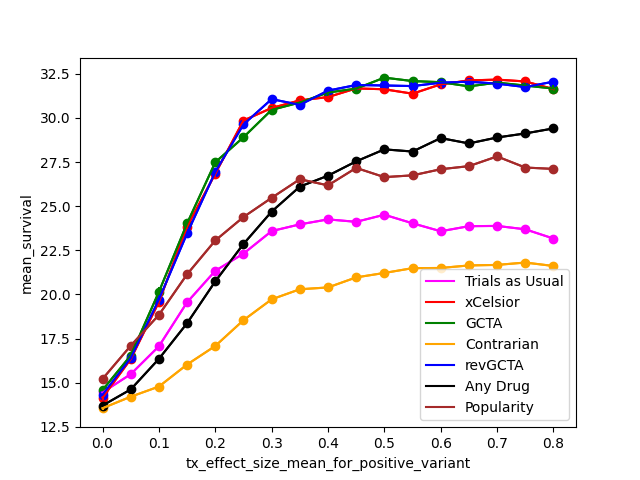
\includegraphics[width=\linewidth]{figs/TheFullMonty=gctaall_n=1000@20210512_0029_303720_x=tx_effect_size_mean_for_positive_variant.png}
  \caption{
    Graphical model representation using plate notation for the Bayesian multilevel model.
  }
  \label{fig:f1}
\end{figure}

\begin{figure}
  \centering
  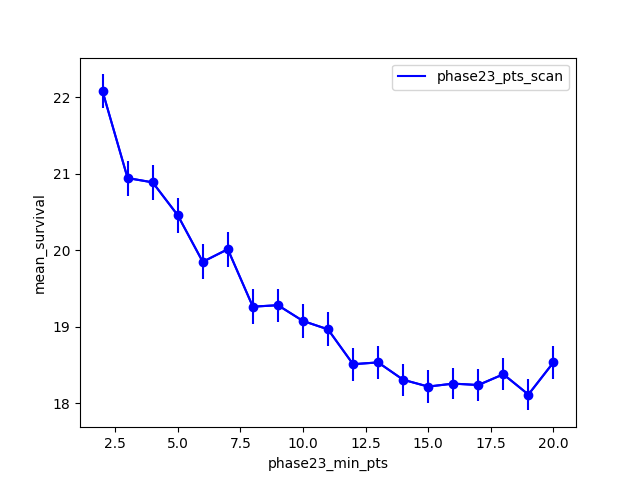
\includegraphics[width=\linewidth]{figs/Phase23_n_patients=phase23_pts_scan_n=1000@20210512_1529_541140_x=phase23_min_pts.png}
  \caption{
    Comparison of simulations from the virtual trial (VT) model to results from a set of randomized controlled trials (RCTs).
  }
  \label{fig:f2}
\end{figure}

\clearpage

\section*{Supplementary materials}
\end{document}

